\documentclass{beamer}

\usepackage{lmodern}
\usepackage{hyperref}
\usepackage{graphicx}

\title{Git gud}
\subtitle{Git voor beginners}
\author{Sticky}
\date{16 februari 2016}

\usetheme{Frankfurt}
\usecolortheme{dove}


% ToC invoegen aan het begin van elke sectie.
\AtBeginSection
{
  \begin{frame}
      \frametitle{Table of Contents}
      \tableofcontents[currentsection]
    \end{frame}
}
% Bron: https://en.wikibooks.org/wiki/LaTeX/Presentations

\begin{document}

\frame{\titlepage}
\frame{
	\frametitle{Slides zelf erbij houden?}
	\url{http://j.mp/gitgudpdf}
}

\section[Get git]{Installatie}

\subsection{Download}
\begin{frame}
	\begin{itemize}
		\item Windows: \url{https://git-scm.com/download/win}
			\begin{itemize}
				\item \small{Maak snelkoppeling naar git-bash in \tt{Program Files/Git/cmd}}
			\end{itemize}
		\item Mac: \url{https://git-scm.com/download/mac}
		\item Linux: gebruik je package manager
	\end{itemize}
\end{frame}

\subsection{Configureren}
\begin{frame}{Instellen (doemoment!)}
	Installeer Git van de site \url{https://git-scm.com}\\

	Open Git Bash en voer in wie je bent:
	\begin{itemize}
		\item \tt{git config --global user.name "Lars Verhoeven"}
		\item \tt{git config --global user.email "user@example.com"}
	\end{itemize}
	{\small\alert{Wordt aan iedere commit verbonden die je maakt!}}\\

	\texttt{git config --global color.ui auto}\\
	\texttt{git config --global core.editor nano}\\

	Als je minder vaak om je wachtwoord wil worden gevraagd (bij externe servers):

	\begin{itemize}
		\item \tt{git config --global credential.helper cache}
		\item \tt{git config --global credential.helper "cache --timeout=3600"}
	\end{itemize}
\end{frame}

\section[Structuur]{Structuur van Git}
\subsection{Locaties}
\begin{frame}
	3 plekken waar je gegevens zitten:\\
	\vspace{.5cm}
	\begin{tabular}{ll}
		 Working directory			& pas je aan, normale map\\
		 Staging area				& bestanden die je gaat committen\\
		 Repository / \texttt{.git/}&Bevat metadata, objecten
	\end{tabular}
	% edit-stage-commit cyclus
\end{frame}

\subsection{Gegevensstructuur}
\begin{frame}{Wat slaat git op?}
	Geen lijst van wijzigingen, maar kopie\"en (snapshots):
	\begin{center}
		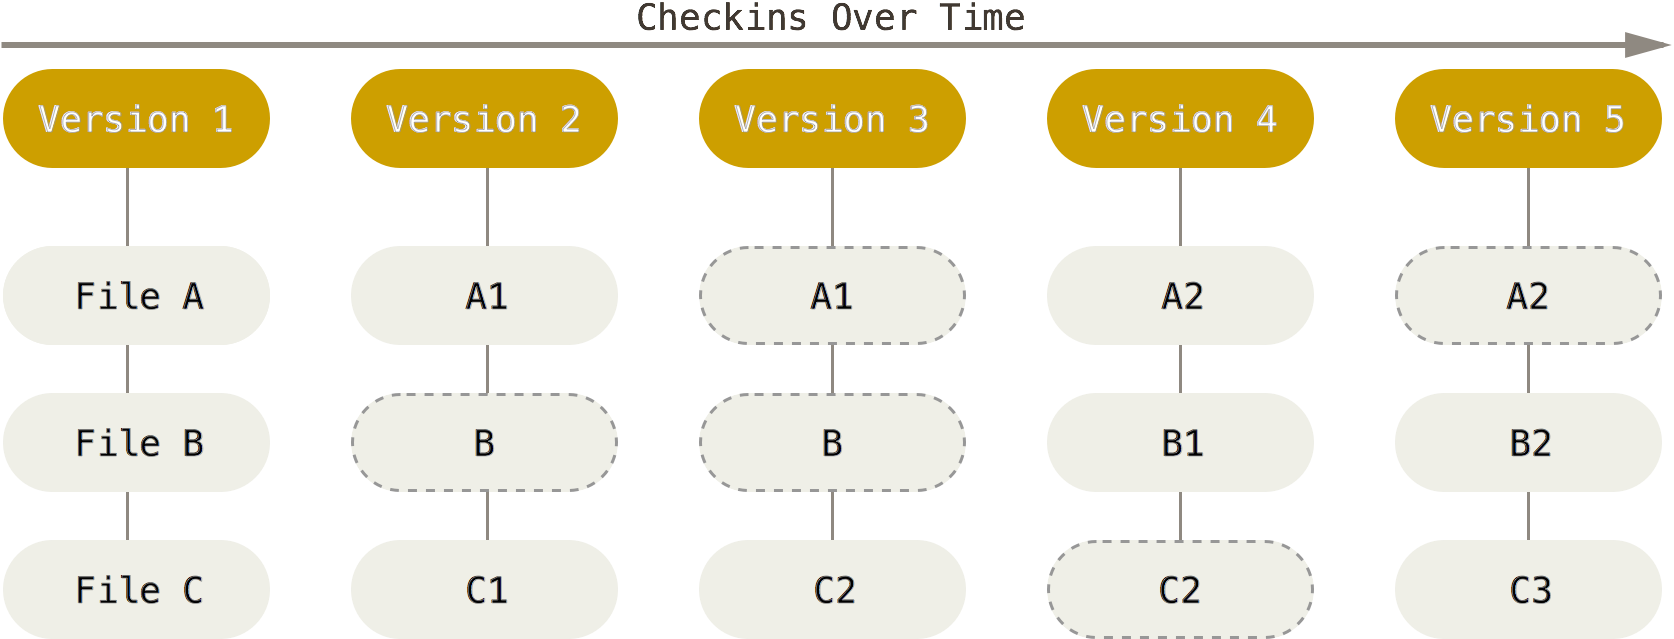
\includegraphics[width=\textwidth]{images/snapshots.png}
	\end{center}
	%(Een version komt hier overeen met een commit, die dus wijst naar versch. versies van bestanden)
\end{frame}

\begin{frame}{Commit}
	\begin{itemize}
		\item Info over jou: (gebruikers)naam + email
		\item Bericht: (hopelijk) korte samenvatting van wat er veranderde
		\item Verwijzing naar set snapshots van bestanden (objects)
		\item Voorganger (merge: 2, initial: 0)
		\item Unieke id (40 tekens)
	\end{itemize}
	\alert{Later (wanneer gedeeld met externe server) niet meer aan (te) passen!}
\end{frame}


\end{document}
